\begin{figure}[htbp]
    \begin{subfigure}{\textwidth}
    \centering
    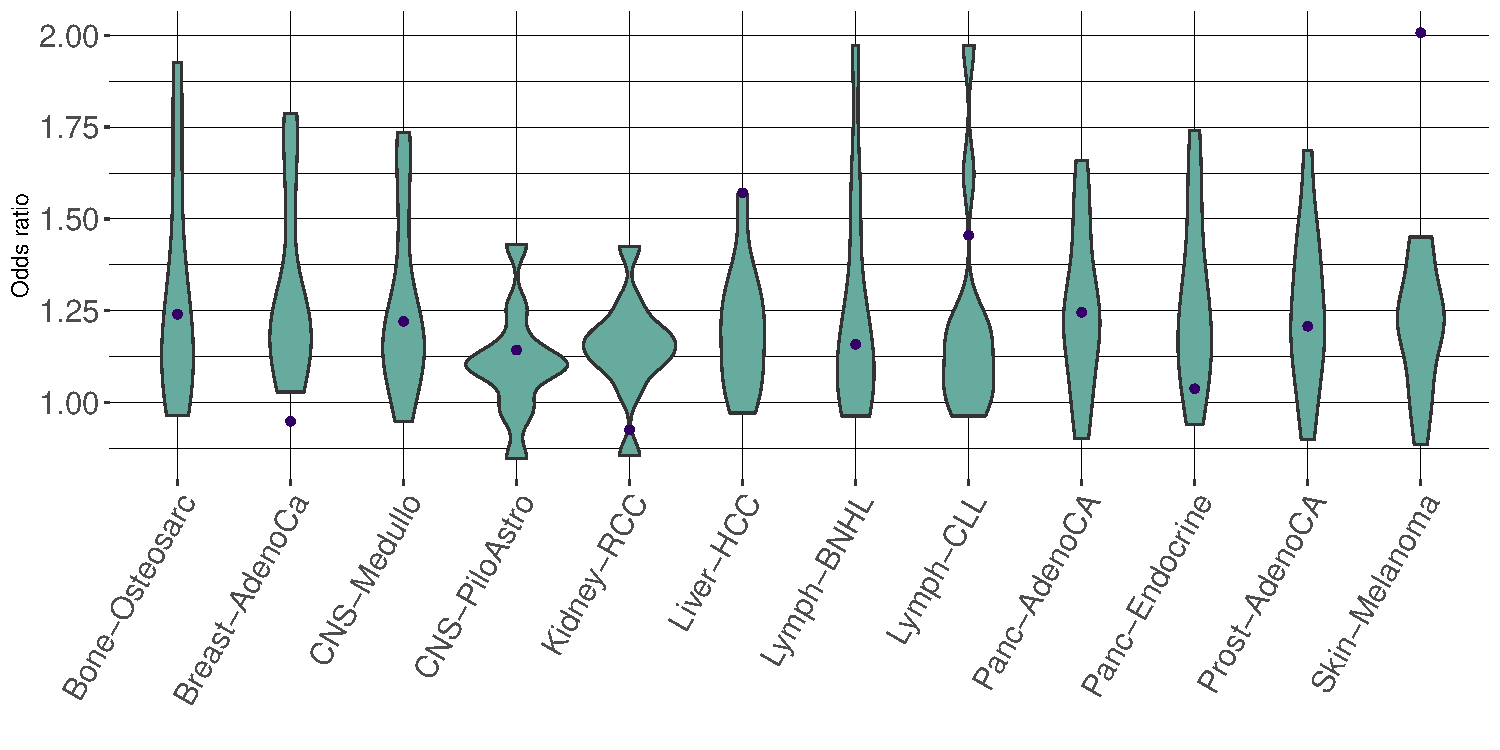
\includegraphics[scale=0.55]{graphics/mixed_or_violin.pdf}
    \caption{violin plot}
    \label{fig:mixed_or_violin}
    \end{subfigure} \\
    
    \vspace{0.2cm}
    \begin{subfigure}{\textwidth}
    \centering
    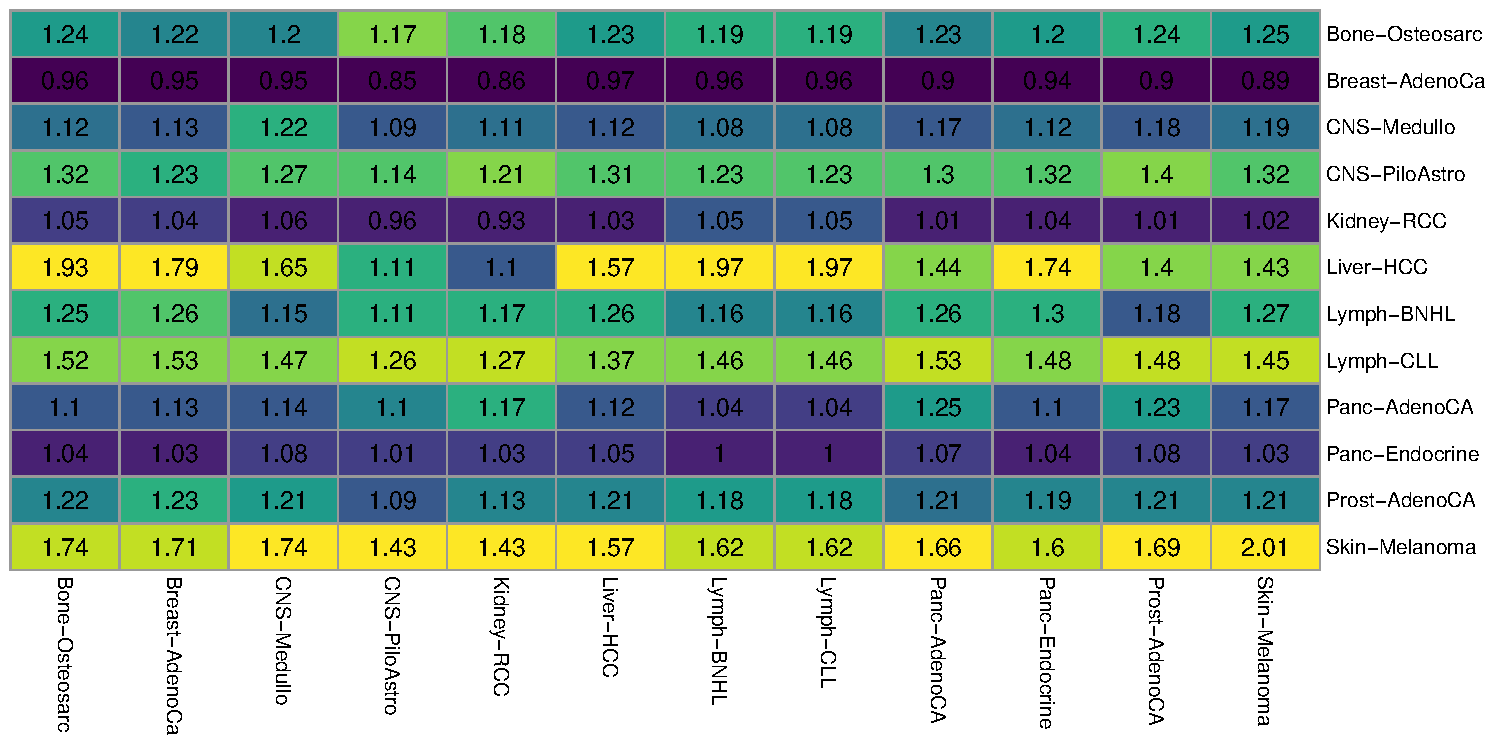
\includegraphics[scale=0.5]{graphics/mixed_or_heatmap.pdf}
    \caption{heatmap}
    \label{fig:mixed_or_heatmap}
    \end{subfigure} 

    \caption{\textbf{The impact of unbalanced DHS data on $OR$ is mild.} This figure shows the (a) violin plot and (b) heatmap of an experiment where $OR$'s were calculated by cross-matching DHS data with mutation data of different cancers. In (a), the x-axis is the cancers whose DHS data was used, the y-axis is the distribution of shuffled $OR$, with the purple dot indicating when mutation data of the true cancer was used. In (b), the column labels are the cancers whose DHS data was used, the row labels are the cancers whose mutation data; each column is coloured by the ranking of $OR$, brighter colours come from cancers whose mutation data produced the greater $OR$'s.}
    \label{fig:mixed_or}
\end{figure}